% Recognition as a basal result of an embodied modulatory network
% Build:  pdflatex main && bibtex main && pdflatex main && pdflatex main
\documentclass[11pt]{article}

\usepackage[margin=1in]{geometry}
\usepackage{graphicx}
\usepackage{amsmath}
\usepackage{booktabs}
\usepackage{microtype}
\usepackage[numbers,sort&compress]{natbib}
\usepackage[colorlinks=true,allcolors=blue]{hyperref}

\graphicspath{{../figures/}}

\title{\textbf{Sensors are not modalities:\\ recognition as a basal result of an embodied modulatory network}}
\author{G.\ Nagarjuna\thanks{IISER Pune, India.} \and Durgaprasad Karnam\thanks{IIT Bombay, India.}}
\date{\today}

\begin{document}
\maketitle

\begin{abstract}
\noindent
Recognising an object---telling it from others---is treated in contemporary AI
as a pattern-classification problem solved by training a neural network on a
labelled corpus. We show that recognition needs no mechanism beyond the basal
architecture of an embodied agent: the same located, opponent-modulated zones
that let a Sensation Modulating Network (SMN) forage also \emph{individuate} an
object, actively and with no labelled data. In a physics-based bench an agent
approaches an object and reads three modalities---touch (whisker angular
extent), vision (rendered luminance), and a chemical ``taste'' field. The number
of objects it can individuate equals $2^{(\text{modalities coupled through
modulation})}$: coupling more modalities multiplies the categories, but adding
more transducers of one modality does not---\emph{sensors are not modalities}.
Discrimination accuracy rises with sensor count only when modulation integrates
the channels; without it, more sensors add nothing---a prediction a trained
classifier would bet against. Locating the object in the agent's own frame
requires reafference, the self/world split. Against the identical task a
subsumption controller (suppression rather than modulation) individuates at most
two categories, and a corpus-trained network needs $\sim$128 labelled examples
to match what the SMN architecture achieves zero-shot. Recognition, on this
account, scales with \emph{modulatory architecture}---not with transducer
richness or a training corpus. All results are reproducible from an open bench.
\end{abstract}

\section{Introduction}

The dominant route to machine recognition is to train a neural network on a
labelled corpus until it maps inputs to class labels. The Sensation Modulating
Network \citep{NagarjunaKarnam2026SMN} suggests a different account: cognition is
what a network of coupled dynamical systems---an embodied agent of sensing,
modulating zones---\emph{does} as it engages its world. A natural first reaction
is to pitch this as ``pattern recognition can be performed by a network of
dynamical systems instead of a neural network.'' That pitch is a trap. It is
already established that recurrent dynamical systems classify---reservoir
computing \citep{Maass2002,JaegerHaas2004}, neural ODEs
\citep{Chen2018NeuralODE}, liquid time-constant networks \citep{Hasani2021Liquid},
and the minimally-cognitive agents of \citet{Beer2003} all recognise as
dynamical systems. Restating that would be neither new nor a contribution, and
it would fight on the classifier's home ground (static input, fixed corpus),
discarding what an embodied architecture actually brings.

We make instead a positive, falsifiable claim about \emph{what} recognition
costs in such an architecture. Three results, all measured on the same bench:

\begin{enumerate}
\item \textbf{Recognition is not a separate competence.} The same located,
  opponent-modulated zones that forage in earlier experiments individuate an
  object---no new module, no new primitive---and they do it \emph{actively},
  driving up to the object and reading it, with no labelled corpus and no
  backpropagation.
\item \textbf{Sensors are not modalities.} What individuates an object is the
  \emph{coupling of distinct modalities through modulation}, not transducer
  richness within one. The number of individuable categories is
  $2^{(\text{modalities coupled})}$; adding more whiskers (more of one
  transducer) does not add categories, and discrimination accuracy rises with
  sensor count only where modulation integrates the channels. This is the
  prediction a trained classifier---for which more input channels are simply
  more features---would bet against.
\item \textbf{The architecture stands in for the corpus.} On the identical task,
  a subsumption controller (fixed-priority suppression rather than modulation)
  individuates at most two categories; a corpus-trained network needs
  $\sim$128 labelled examples to reach what the SMN architecture achieves
  zero-shot. And locating the object in the agent's own frame requires
  reafference---the self/world split.
\end{enumerate}

The contribution is therefore not ``dynamical systems can recognise too,'' but
\emph{recognition scales with modulatory architecture, not with transducer count
or a labelled corpus}---and a concrete, reproducible demonstration of it.

\section{Related work}

\paragraph{Recognition by dynamical systems.}
That a recurrent dynamical system can categorise is not in question. Reservoir
computing reads a class off the trajectory of a perturbed dynamical reservoir
\citep{Maass2002,JaegerHaas2004}; neural ODEs and liquid time-constant networks
are classifiers that are literally continuous-time dynamical systems
\citep{Chen2018NeuralODE,Hasani2021Liquid}. Closest to us,
\citet{Beer2003} evolved continuous-time recurrent agents that perform
\emph{active categorical perception}---catching some shapes, rejecting others.
Our point of departure from this lineage is specific: we do not evolve or train
a network to the task, and our discriminating mechanism is the \emph{modulatory
coupling of multiple modalities} (with opponent zones and a self/world split),
not a single recurrent substrate optimised end-to-end.

\paragraph{Embodiment without a dataset.}
\citet{Brooks1991} argued for intelligence without representation: layered
reactive behaviours, no labelled world model. The SMN keeps that no-dataset,
embodied commitment but replaces \emph{suppression} (a higher layer overriding a
lower one) with \emph{modulation} (graded, antagonistic coupling that binds
channels), and it does build a constructed, body-relative snapshot. Subsumption
historically hit a ceiling at higher cognition; we show below, as a measured
arm, exactly where suppression stalls. \citet{PfeiferBongard2006} on
morphological computation is an ally: much of what looks like computation is paid
for by the body and its coupling---here, by the modulatory architecture and the
cross-modal convergence it affords. Our reading of perception as constituted in
sensorimotor engagement follows the enactive/sensorimotor tradition
\citep{ORegan2001} and Gibson's affordances \citep{Gibson1979}; interactive
perception in robotics \citep{Bohg2017} similarly leverages action, typically
still atop learned perception.

\section{The bench and the cross-modal architecture}

The experiments run on \texttt{smn-lab}, an open MuJoCo bench in which the SMN
control architecture drives a physical body \citep{NagarjunaKarnam2026SMN}. A
planar agent (a ``mouse'') has translational and yaw degrees of freedom, a fan of
rangefinder whiskers, a forward-facing camera, and an inertial site for
proprioception. Locomotion is produced by a basal action pattern (a central
pattern generator) and two \emph{located} opponent drive zones whose net force
and torque follow from the body geometry---so the controller that forages in
prior experiments is, unchanged, the controller that approaches here.

The object to be recognised carries one feature bit per modality
(Figure~\ref{fig:main}, right): its \textbf{radius} sets the tactile bit (a bigger
object subtends more whiskers at a fixed gap); its \textbf{luminance} sets the
visual bit, read from the rendered camera image pooled into patch tokens; and a
Gaussian chemical field at the object sets the \textbf{taste} bit, sampled where
the agent stands (so it must approach to taste). With three bits there are eight
object types.

The independent variable is the \emph{cross-modal board}---the experiment's
``balance beam.'' It (a) \emph{modulates}: each modality's reading is gated
against a noise floor, so only a reading that breaks the floor flows; and
(b) \emph{couples}: the surviving bits of the wired-in modalities are
concatenated into one object code. The visual channel is surfaced by
\emph{reafference}: at closest approach a small forward probe makes the object
loom in a way the agent's rotation-only forward model cannot predict, and the
modulator gates the unpredicted change---figure-ground from the agent's own
motion. Localisation places the object in the agent's dead-reckoned frame, built
from proprioception rather than any absolute pose.

\section{Results}

We report four measurements. Binding, localisation, and the foils run on the
embodied bench (one object per trial; the agent approaches and reads at closest
approach). The resolution sweep is a controlled Monte-Carlo isolating the
integration principle. All randomness is seeded; the experiment and figures are
regenerable from a single script.

\begin{figure}[t]
  \centering
  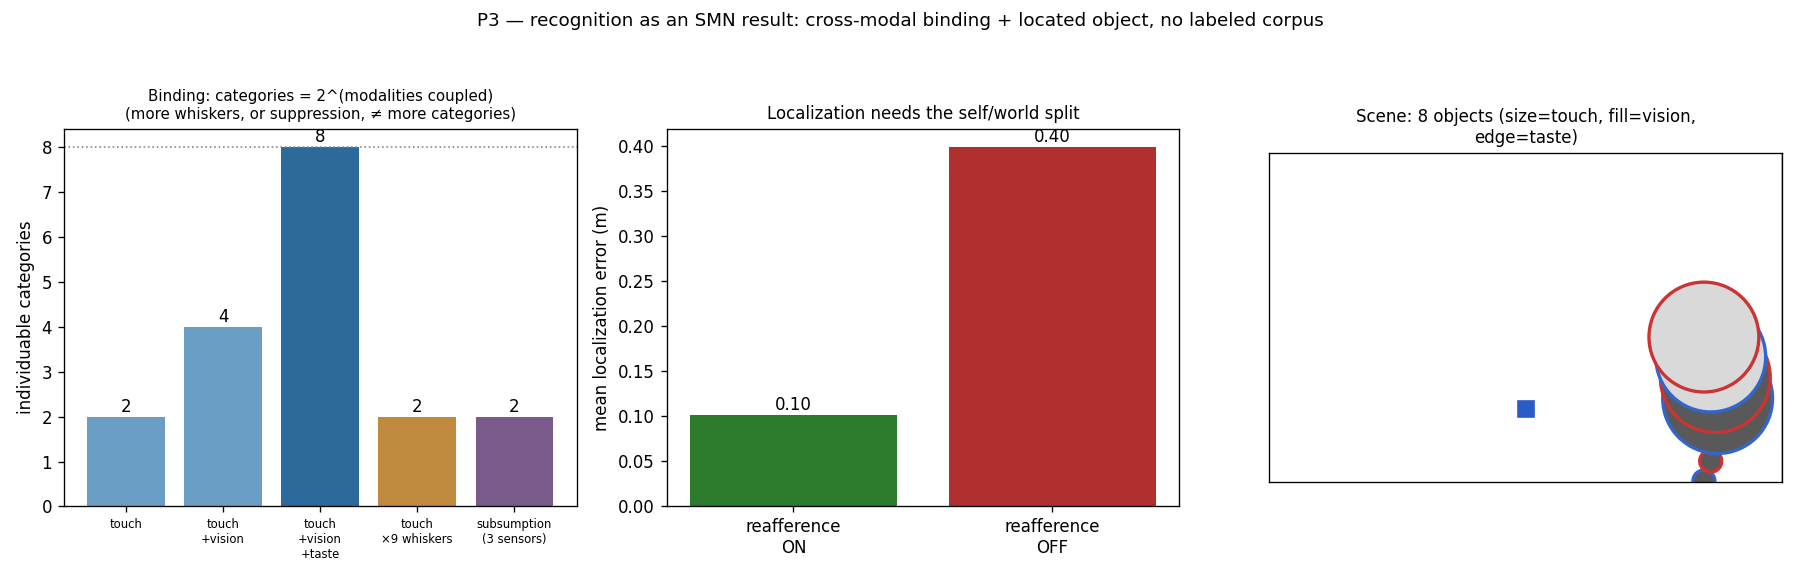
\includegraphics[width=\linewidth]{p3_crossmodal_discrimination.png}
  \caption{\textbf{Binding and localisation.} \emph{Left:} individuable
  categories $=2^{(\text{modalities coupled})}$ ($2\!\to\!4\!\to\!8$); a
  touch-only agent with nine whiskers still individuates only two, and a
  subsumption controller with all three sensors also only two---neither
  transducer density nor suppression adds categories. \emph{Centre:} mean
  localisation error is $\sim$5$\times$ worse without reafference, and
  approximates the distance the agent travelled---the signature of attributing
  self-motion to the world. \emph{Right:} the eight objects (size$=$touch,
  fill$=$vision, edge$=$taste).}
  \label{fig:main}
\end{figure}

\subsection{Binding: the object is a cross-modal invariant}

Decoding all eight objects with the cross-modal board, the number of
individuable categories equals $2$ raised to the number of modalities coupled
through modulation: \textbf{2} (touch) $\to$ \textbf{4} (touch$+$vision) $\to$
\textbf{8} (touch$+$vision$+$taste), with every resolved bit correct
(Figure~\ref{fig:main}, left). One modality collapses the set fourfold; coupling
individuates. Crucially, giving the touch-only agent \emph{nine} whiskers instead
of five leaves it at \textbf{2} categories: a touch-only agent cannot read colour
no matter how many whiskers it grows. The empirical content is the dissociation,
not the multiplication---\emph{sensors are not modalities}.

\subsection{The resolution principle: modulation, not sensor count}

\begin{figure}[t]
  \centering
  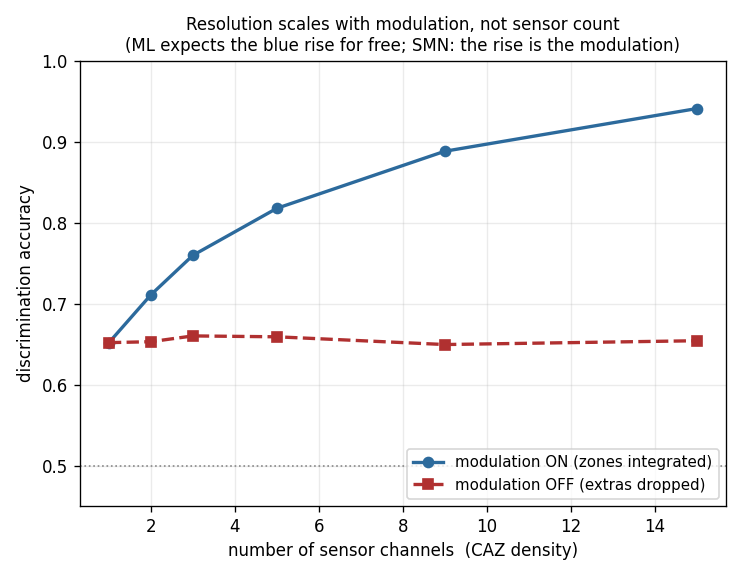
\includegraphics[width=0.62\linewidth]{p3_resolution_principle.png}
  \caption{\textbf{Resolution scales with modulation, not sensor count.} With
  $N$ redundant noisy channels, modulation integrates the gated zones and
  accuracy rises as $\sigma/\sqrt{N}$ (0.65$\to$0.94); strip the modulation and
  the ungated extras are dropped, so more sensors are flat ($\approx$0.65). A
  trained classifier expects the rising curve from raw channels for free; the
  SMN claim is that the rise is bought by the modulatory architecture.}
  \label{fig:resolution}
\end{figure}

Why does density within a modality not help? Because resolution is a function of
the modulatory architecture, not of the raw transducer. In a controlled
two-class discrimination from $N$ redundant noisy channels
(Figure~\ref{fig:resolution}), \emph{with} modulation the modulator integrates
the gated zones and accuracy climbs from $0.65$ ($N{=}1$) to $0.94$ ($N{=}15$)
as $\sigma/\sqrt{N}$; \emph{without} modulation the ungated extras are dropped
and accuracy is flat ($\approx 0.65$) regardless of $N$. The rise is not a
property of having more sensors---it is bought by the architecture that
integrates them. This is precisely the prediction a feature-hungry classifier
would bet against.

\subsection{Localisation needs reafference}

The agent reports not just \emph{what} the object is but \emph{where}, in its own
dead-reckoned frame---so the world model includes locating objects in space.
Holding the object at a stable place while the agent moves toward it requires
discounting self-caused sensory change. With reafference on, mean localisation
error is $\sim$\,0.10\,m; with it off, $\sim$\,0.40\,m---roughly the distance the
agent travelled, because the agent then attributes its own approach to the object
(Figure~\ref{fig:main}, centre). The self/world split is not an add-on to
recognition; it is what makes the located object stable.

\subsection{Foils: the architecture against suppression and against a corpus}

\begin{figure}[t]
  \centering
  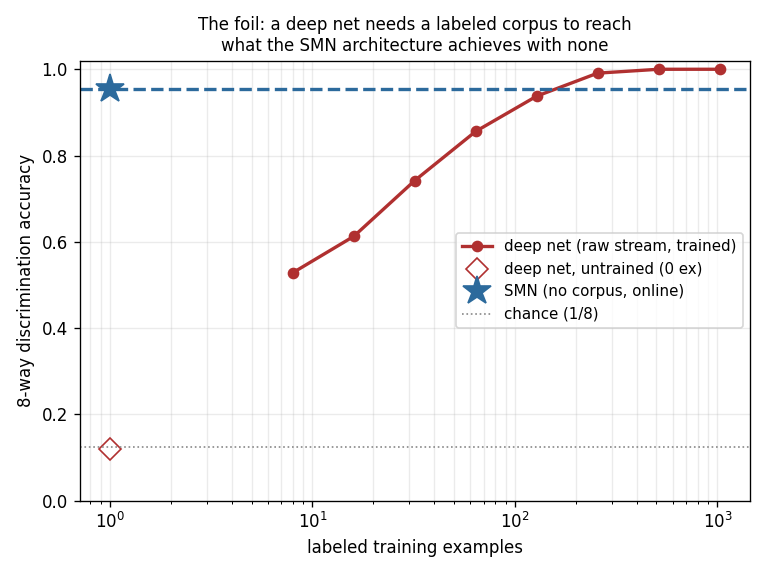
\includegraphics[width=0.62\linewidth]{p3_deepnet_foil.png}
  \caption{\textbf{The architecture stands in for the corpus.} On the same
  generative test set, an untrained network sits at chance ($\sim$0.12) and the
  SMN architecture scores $\sim$0.96 with \emph{zero} labelled examples; a
  trained network needs $\sim$128 labelled examples to match it. At the same zero
  corpus the gap is the whole distance from chance to near-perfect.}
  \label{fig:foil}
\end{figure}

We compare the SMN architecture to its two natural foils on the identical task
(Table~\ref{tab:foils}). The \emph{subsumption} foil shares the body, the three
sensors, and the reactive approach, but arbitrates by fixed-priority
\emph{suppression} rather than modulation: the highest-priority firing layer
suppresses the rest and emits one bit. Because suppression replaces rather than
binds, it individuates at most \textbf{2} categories with all three sensors
present---the ceiling that modulation breaks through to 8. The \emph{deep-net}
foil is a small network trained on the raw sensory stream (whisker ranges,
camera tokens, taste). On a generative test set drawn from the same per-object
readings plus channel noise, an untrained network sits at chance ($\sim$0.12,
$1/8$) and a trained one reaches the SMN architecture's zero-shot accuracy
($\sim$0.96) only after $\sim$128 labelled examples (Figure~\ref{fig:foil}). What
a network must learn from a corpus, the SMN architecture supplies as an embodied
prior.

\begin{table}[t]
  \centering
  \small
  \begin{tabular}{lcc}
    \toprule
    System (all three sensors) & Labels & Categories / accuracy \\
    \midrule
    SMN (cross-modal board)          & 0          & 8 \ ($\sim$0.96 on the noisy set) \\
    Subsumption (suppression)        & 0          & 2 \\
    Deep net (untrained)             & 0          & $\sim$0.12 (chance) \\
    Deep net (trained)               & $\sim$128  & $\sim$0.96 (matches SMN) \\
    \bottomrule
  \end{tabular}
  \caption{The same task, three systems. Modulation binds (8); suppression does
  not (2); a trained network matches SMN only after a corpus.}
  \label{tab:foils}
\end{table}

\section{Discussion}

Across the four measurements a single point recurs: \emph{the modulatory
architecture is doing the work that classifiers buy with data}. Recognition is
not a competence layered on top of the agent---it is what the basal, located,
opponent-modulated zones already do when coupled across modalities. The
recognised category is the equivalence class of scenes that drive the same
coupled code; the object is the cross-modal invariant, determinate where distinct
modalities, coupled through modulation, agree. Resolution is architectural, not a
function of transducer count; and locating the object requires the same
self/world split the agent uses to map. None of this needs a new mechanism or a
labelled corpus.

The account is deliberately bounded. \emph{Naming}---mapping an object code to an
utterance---is another modulatory coupling, but a name is conventional and
social: it requires at least a dyad, and is the subject of the next monograph in
this programme rather than of this paper. The encounter here is staged one object
at a time for a controlled read; recognition emerging during open foraging is a
natural next step. And the reafference gate uses a rotation-only forward model,
so it surfaces the object from self-caused translation it cannot yet predict---a
figure-ground signal, not yet a model that predicts looming. The strength of the
result is what it refuses to claim: a single, falsifiable dissociation
(sensors~$\neq$~modalities; architecture~$\neq$~corpus) demonstrated end to end.

\section{Reproducibility}

The bench, the experiment, and an interactive lab interface are open
(\texttt{github.com/gnowgi/smn-lab}, GPL-3.0). Every result above is produced by
a single seeded script (\texttt{experiments/\allowbreak
p3\_crossmodal\_\allowbreak discrimination.py}); the three figures regenerate from it. A Streamlit interface lets a reviewer run
the controller live---watch the agent approach and read each object, and compute
the result tables on the spot---so the figures are visibly the math in action
rather than reported numbers. A versioned snapshot with a Zenodo DOI will
accompany the published version.

\section{Conclusion}

Recognition, in an embodied Sensation Modulating Network, is a basal result: the
same modulatory zones that keep the agent alive individuate an object, actively
and without a corpus. What individuates is the coupling of modalities through
modulation, and what makes the object's place stable is reafference. The clear,
contestable claim---\emph{recognition scales with modulatory architecture, not
with transducer richness or a labelled corpus}---is borne out by a measured
dissociation against both suppression and a trained network. Sensors are not
modalities; architecture is not a corpus.

\bibliographystyle{plainnat}
\bibliography{references}

\end{document}
